\documentclass[]{article}

\usepackage{enumitem}
\usepackage{listings}
\usepackage[margin=1in]{geometry}
\usepackage{courier}
\usepackage{indentfirst}
\usepackage{graphicx}
\usepackage{mdframed}
\lstset{basicstyle=\footnotesize\ttfamily,breaklines=true}

%opening
\title{Noteworthy Features of the Average Joes' 2015 FRC Code}
\author{Doug Wegscheid}

\begin{document}

\maketitle

\begin{abstract}

FRC Team 3620, "The Average Joes", from St.\ Joseph High School in St.\ Joseph, Michigan, is releasing their 2015 Java code for other FRC teams to learn from.
The code is available on github:
\\
\texttt{https://github.com/FRC3620/FRC3620\_2015\_AverageJava}

This paper is a summary of what the team programming mentor considers to be features that other FRC teams may want to look at and use: event logging, data logging, UDP transmission to an onboard co-processor, UDP reception from an onboard co-processor, and adding third party jars to the build.

Some of the information contained here was not discovered or developed by The Average Joes; much of it was gleaned from other team's postings of code, discussions on Chief Delphi, or other publicly available sources.
We didn't generally keep track of where we got ideas that we reused, and apologize for not being to  attribute them properly.

\end{abstract}

\section{Overview}

Our 2015 FRC programming was done in Java command-based code, using RobotBuilder.
We did version control with git, using github as our central repository.

The code was developed by Ved Ameresh (a junior), Patrick Fischer (a junior), Mike Miller (a senior, now at Michigan Technological University), Steve Sykora (a senior, now at Calvin College in Grand Rapids, Michigan), and myself.

There are 5 features of the 2015 code that may be of use to other teams:

\begin{itemize}[topsep=0pt]

\item event logging

Event logging is the timestamped logging to a file of significant events during the execution of robot code.
Events worth logging could include:
\begin{itemize}[noitemsep,topsep=0pt]
\item transitions between autonomous, teleop, test, and disabled states.
\item initialization, end, and interruption of commands.
\item blockage of operation because of limit switches.
\item acquisition and loss of vision targets.
\item brownouts.
\item selection of different autonomous modes.
\end{itemize}

Figure~\ref{fig:eventlog} is an example of an event log.
\begin{figure}[h]
\begin{mdframed}
\begin{lstlisting}[basicstyle=\ttfamily\tiny]
2015/04/23 12:16:59.840 [org.usfirst.frc3620.Robot] INFO - Moving from DISABLED to AUTONOMOUS, position = Blue 1, FMS = true
2015/04/23 12:16:59.850 [org.usfirst.frc3620.Robot] INFO - Using autonomous autonomous (prefs were Tote and bin )
2015/04/23 12:16:59.866 [org.usfirst.frc3620.Robot] INFO - Command init: liftManual
2015/04/23 12:16:59.869 [org.usfirst.frc3620.Robot] INFO - Command init: DriveArcadeCommand
2015/04/23 12:16:59.906 [org.usfirst.frc3620.Robot] INFO - Command interrupt: liftManual
2015/04/23 12:16:59.912 [org.usfirst.frc3620.Robot] INFO - Command interrupt: DriveArcadeCommand
2015/04/23 12:16:59.939 [org.usfirst.frc3620.Robot] INFO - Command init: intakeClose
2015/04/23 12:16:59.942 [org.usfirst.frc3620.Robot] INFO - Command end:  intakeClose
...
2015/04/23 12:17:15.199 [org.usfirst.frc3620.Robot] INFO - Moving from AUTONOMOUS to DISABLED, position = Blue 1, FMS = true
2015/04/23 12:17:15.203 [org.usfirst.frc3620.Robot] INFO - Command interrupt: liftManual
2015/04/23 12:17:15.205 [org.usfirst.frc3620.Robot] INFO - Command interrupt: DriveArcadeCommand
2015/04/23 12:17:15.758 [org.usfirst.frc3620.Robot] INFO - Moving from DISABLED to TELEOP, position = Blue 1, FMS = true
2015/04/23 12:17:15.763 [org.usfirst.frc3620.Robot] INFO - Command init: liftManual
2015/04/23 12:17:15.767 [org.usfirst.frc3620.Robot] INFO - Command init: DriveArcadeCommand
2015/04/23 12:17:36.443 [org.usfirst.frc3620.Robot] INFO - Command init: takeIn
2015/04/23 12:17:38.404 [org.usfirst.frc3620.Robot] INFO - Command init: intakeOpenClose
2015/04/23 12:17:38.407 [org.usfirst.frc3620.Robot] INFO - Command end:  intakeOpenClose
2015/04/23 12:17:40.068 [org.usfirst.frc3620.Robot] INFO - Command interrupt: takeIn
...
2015/04/23 12:19:34.283 [org.usfirst.frc3620.Robot] INFO - Moving from TELEOP to DISABLED, position = Blue 1, FMS = true
2015/04/23 12:19:34.289 [org.usfirst.frc3620.Robot] INFO - Command interrupt: liftManual
2015/04/23 12:19:34.292 [org.usfirst.frc3620.Robot] INFO - Command interrupt: DriveArcadeCommand
\end{lstlisting}
\caption{Event log sample}
\label{fig:eventlog}
\end{mdframed}
\end{figure}

One of our requirements was that all logging be done at the roboRIO (not the driver station PC, which would consume valuable bandwidth).

\item data logging

Data logging is the continuous timestamped logging of significant sensor data, actuator status, power statistics (voltage and current draw), and operator inputs to a file.
This data could be processed after a test session, practice session, or match using Excel, Veusz, gnuplot, or some other graphics or analytical software to provide plots of such data.
Figure~\ref{fig:datalog} is an example of such a data log.

\begin{figure}[h]
\begin{mdframed}
\begin{lstlisting}[basicstyle=\ttfamily\tiny]
time,timeSinceStart,robotMode,robotModeInt,rightDriveCurrent,rightDriveMotorPower,leftDriveCurrent,leftDriveMotorPower,liftMotorCurrent,compressorCurrent
04-23-2015 13:25:00.985,0,DISABLED,1,0.0,0.0,0.0,0.0,0.0,0.0
04-23-2015 13:25:02.05,1020,DISABLED,1,0.0,0.0,0.0,0.0,0.0,0.0
...
04-23-2015 13:25:08.103,7118,DISABLED,1,0.0,0.0,0.0,0.0,0.0,0.0
04-23-2015 13:25:09.183,8198,AUTONOMOUS,2,0.0,-0.0038314176245210726,0.0,-0.0038314176245210726,0.0,0.0
04-23-2015 13:25:10.205,9220,AUTONOMOUS,2,0.0,-0.0038314176245210726,0.0,-0.0038314176245210726,0.0,0.0
...
04-23-2015 13:25:23.464,22479,AUTONOMOUS,2,0.0,-0.0038314176245210726,0.0,-0.0038314176245210726,0.0,0.0
04-23-2015 13:25:24.484,23499,DISABLED,1,0.0,-0.0038314176245210726,0.0,-0.0038314176245210726,0.0,0.0
04-23-2015 13:25:25.507,24522,TELEOP,3,0.0,-0.0038314176245210726,0.0,-0.0038314176245210726,0.0,0.0
\end{lstlisting}
\caption{Data log sample}
\label{fig:datalog}
\end{mdframed}
\end{figure}

We used this data in 2015 to determine if it was possible to lose weight by changing to a smaller air compressor.
We logged the current drawn by the compressor, and by looking at the plot of current draw, we were able to determine exactly how much the compressor was run during any given match. See Figure~\ref{fig:plot}.

\begin{figure}[h]
\begin{mdframed}
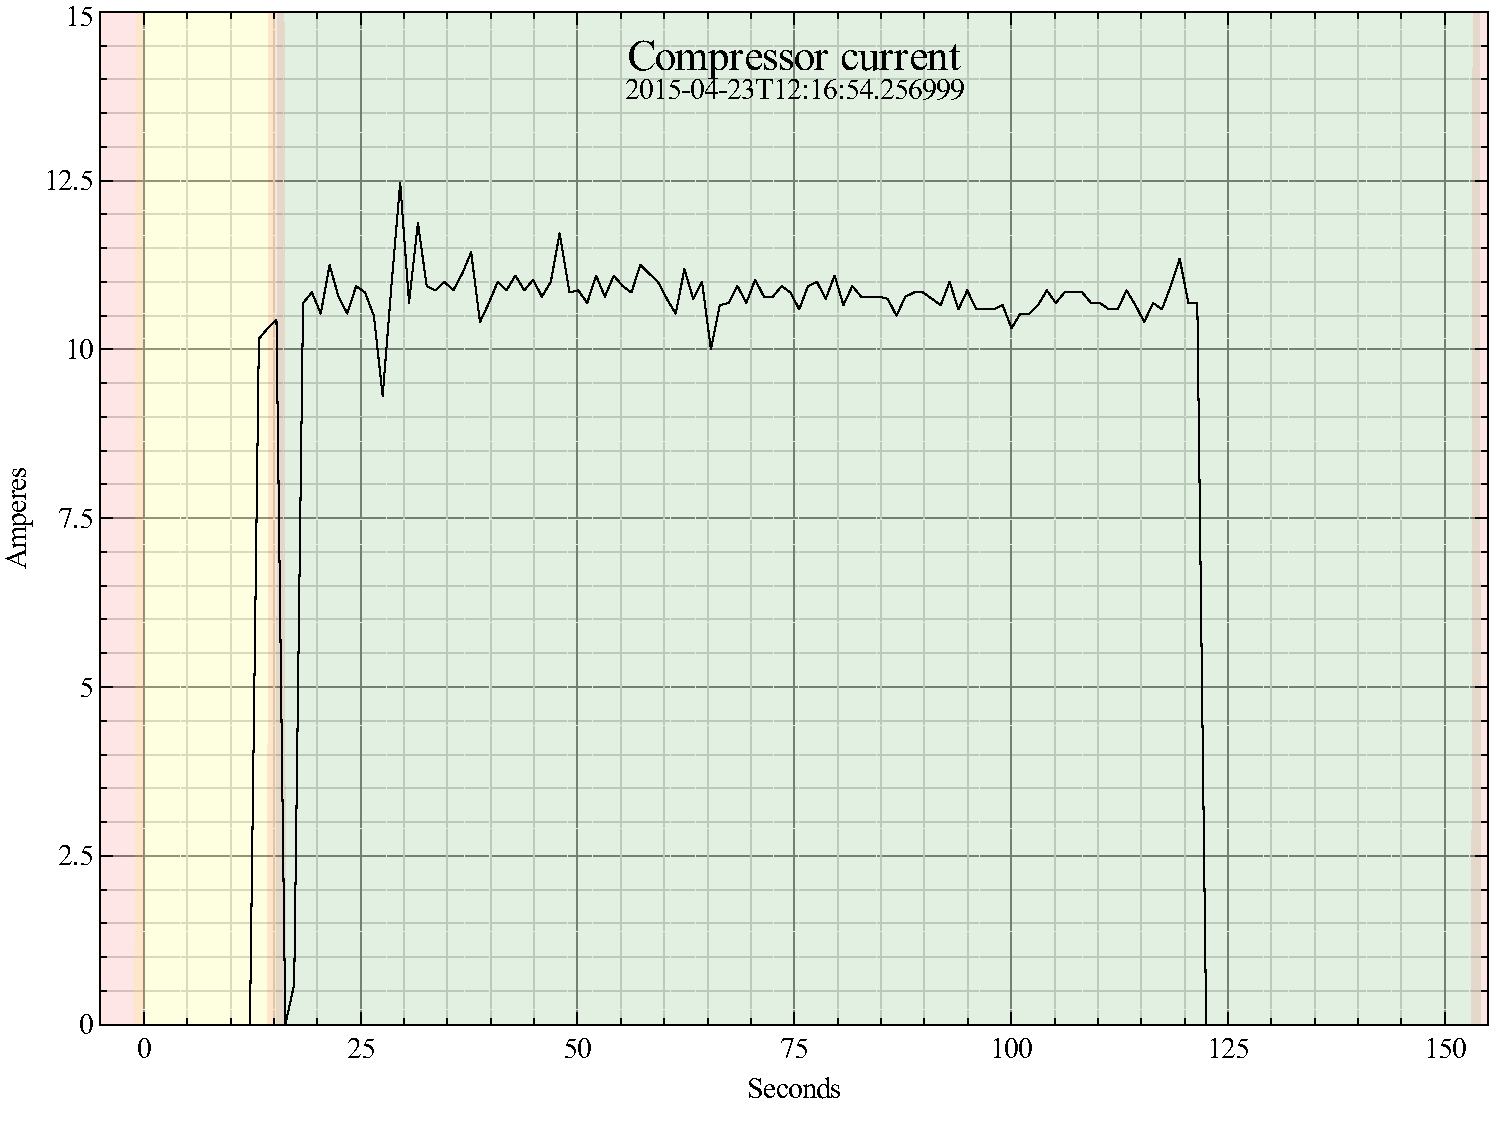
\includegraphics[width=6in]{Plots3.pdf}
\caption{Veusz plot of compressor current data}
\label{fig:plot}
\end{mdframed}
\end{figure}

\item UDP reception from onboard co-processor

Our original plan for vision was to do vision processing on a Raspberry Pi, using a Python script calling OpenCV.
We did have demonstrable ability to detect and track yellow totes.

We needed to send the coordinates, size, and presence of the target back to the roboRIO for use during autonomous mode. Sending JSON over UDP seemed to be a light solution\footnote{
This could have been done using network tables, but we were not (at the time) aware of pynetworktables written by Peter Johnson of FRC Team 294 and Dustin Spicuzza of  FRC Team 1418/2423.
Running a side by side comparisons of CPU and network utilization using the two approaches would be a good 2016 activity.}, and we implemented that.

We ended up not needing vision capability, so code that exercised it was disabled.

\item UDP transmission to onboard co-processor

After we decided that we didn't need to do vision processing, we decided to use the OpenCV knowledge we had learned to make a video recording of the match with information from the roboRIO overlaid on the video.
To accomplish this, we need to periodically transmit some data from the roboRIO to the Raspberry Pi.

The data was encoded to JSON, then sent via UDP.

\item Adding third-party jar files to the build

In the mentor's professional experience, the SLF4J API has shown significant advantages over the native java.util.logging APIs.
The SLF4J APIs are not part of the Java runtime, and typically are loaded from a library jar.
We were able to modify the build.properties used to build the roboRIO's jar file to include the SLF4J APIs so that we could use them.

\end{itemize}

\section {Log File Naming and Location}

One of our requirements for logging was that the event and data logs should be placed in the same directory (on a thumb drive, if one is inserted in the roboRIO), and have the same name (but different file types).
The filename format we decided on was based on the current time, and was formatted "yyyyMMdd-HHmmss" (which sorts correctly).
For simplicity (and because none of our matches spanned any Daylight Savings Time "spring forwards" or "fall backs") we decided to format the date and time using the Eastern Time Zone, where all our practices and matches took place (except for CMP). We considered using GMT (commonly used in industry because of it's unambiguous nature and lack of glitches around DST changes), but those advantages had no value here, and were offset by the disadvantage of having to do timezone conversion when trying to find the files for a particular time.

New data and event log files (with new names) are written every time the robot code is restarted (at roboRIO boot, user code load, or user code restart). If multiple practice matches are played in a row, with no intervening roboRIO restarts, the data for all the matches will be in the same data and event logs.

The roboRIO has no onboard realtime clock; the system clock appears to start at Linux epoch time 0 (January 1, 1970) when the roboRIO is booted.
The system clock apparently is initialized to the driver station current time sometime during the establishment of communications between the driver station and the roboRIO.
Until that initialization takes place, the roboRIO has no idea of the current time, and cannot determine the correct file name. We made the decision to just not log data or events until that occurs.

The filename is derived from the system time at the instant of the first data or event logging that takes place after the system clock is set. 

Method getTimestampString() in class org.usfirst.frc3620.LogTimestamp contains the code that determines the filename for the data and event logs; getTimestampString() will return a null if the system clock has not yet been sent, else it provides the "yyyyMMdd-HHmmss" data.
Once getTimestampString() has determine the correct name to use, the name is cached so that calls to determine event and data log file names return the same result, even though the calls happen at different times.

The code to determine the directory to put the data and event logs into is in the robotInit() method of org.usfirst.frc3620.Robot.
It looks for a thumbdrive with a writable "logs" directory; if none is found, logging will go to /home/lvuser/logs.

\section {Event Logging}

We used the JRE provided java.util.logging framework to do the actual logging\footnote {
We considered using Apache log4j 2 instead of java.util.logging, but log4j has dependencies on parts of the Java runtime that are not present in the compact version of the Java runtime that FIRST has us install on the roboRIO.
}, but used the SLF4J logging API as our mechanism to getting log events into java.util.logging.
If the runtime on the roboRIO becomes complete enough to support log4j2, we would be able to use that (with it's configuration and performance advantages over j.u.l), and keep the same logging statements that we have always used.

Method setup() in class org.usfirst.frc3620.EventLogging contains the code for programmatically setting up java.util.logging.
It sets up a console handler (so that logged messages go to Riolog), and also sets up a custom file handler.
The custom file handler will silently ignore logging attempts until it is able to get a valid log file name from LogTimestamp.
EventLogging also has a custom event formatter that formats the events reasonably concisely.

EventLogging has some useful convenience methods:
writeToDS will write a message to the message area of the FRC Driver Station, and exceptionToString makes a reasonably concise formatting of an exception.

EventLogging also has a convenience method for getting an org.slf4j.Logger object for a class, and setting it up for the desired logging level.
Use of this can be seen in the org.usfirst.frc3620.VideoFeeder class.
java.util.logging is typically configured by using a configuration file and specifying the name of that configuration file on the java command line, or by passing the configuration into the readConfiguration() method of java.util.logging.LogManager.
We rejected this because it required students that were debugging to make changes in both the modules they were debugging and the central log configuration.
We finally landed on this compromise where the logging level for a module was set in the module's code when creating the logger for that module.

Development of the event logging was taking place at the same time as the rest of the development, so it was not well utilized in our 2015 code.

\section {Data Logging}

Data logging was taken care of in class org.usfirst.frc3620.DataLogger.

At the end of execution of any *periodic() method\footnote{disabledPeriodic(), autonomousPeriodic(), teleopPeriodic(), or testPeriodic()} a check is done to see if it's been "long enough" since the last data logging took place, and if so, name-value pairs are placed in the DataLogger and written out in CSV format.
The DataLogger does not keep track of what names are in what columns, so care needs to be taken to always call addDataItem with the name-value pairs in the same order. 

The use of the DataLogger can be found in the allEndOfPeriodic() method in org.usfirst.frc3620.Robot.

2016 improvemenst to the DataLogger could be limiting the number of significant digits stored (to save space), using an off the shelf CSV formatter, and removing the restriction that calls to addDataItem are always made in the same order.

\section {UDP reception from onboard co-processor}

Class org.usfirst.frc3620.UDPReciever contains the code for receiving UDP packets from the Raspberry Pi, decoding the JSON contained in them, and make the resultant object available in a static variable for use by other classes.
I believe this code was lifted bodily from an example on the Internet involving stock quotes.

Use was simply instantiating a UDPReciever object, and calling it's start() method; see the robotInit() method in org.usfirst.frc3620.Robot.

The error handling in UDPReciever is \textbf{not} robust.

For conversion from JSON, we just used the Google GSON library; it was small, simple, and had no dependencies on anything besides the Java runtime.
At the time this work was done, we didn't know how to include third-party jars, so we just imported the source code into our project. 

\section {UDP transmission to onboard co-processor}

Class org.usfirst.frc3620.VideoFeeder contains the code for collecting data needed by the video recording application on the Raspberry Pi, encoding it into JSON, and sending it via UDP.
The VideoFeeder sent the filename being used by the data and event logging over to the Raspberry Pi, so that the video files generated there would have the same names as the corresponding log files on the roboRIO.

It is started by simply instantiating a VideoFeeder object.

\section {Adding third-party jar files to the build}

Adding third-party jar files for the SLF4J libraries to the build ended up being simple; it just involved setting the "classpath" property in build.properties.

There is a master build.properties file in the java/current/ant folder of the wpilib.
That master file has classpath defined as
\begin{lstlisting}[frame=single]
classpath=${wpilib.jar}:${networktables.jar}
\end{lstlisting}

We can override this in the project-specific properties file, but any variables used in the override must also be defined in the project-specific properties file.
We ended up having to copy the definitions of \$\{wpilib.jar\} and \$\{networktable.jar\}. Our build.properties has those definitions (as well as a couple of unneeded ones, it appears). The necessary bit would be:
\begin{lstlisting}[frame=single]
wpilib=${user.home}/wpilib/java/${version}
wpilib.lib=${wpilib}/lib
wpilib.jar=${wpilib.lib}/WPILib.jar
networktables.jar=${wpilib.lib}/NetworkTables.jar
classpath=lib/slf4j-api-1.7.10.jar:lib/slf4j-jdk14-1.7.10.jar:${wpilib.jar}:${networktables.jar}
\end{lstlisting}

\end{document}
